\documentclass[oneside,a4paper,14pt]{extarticle}
\usepackage[T1,T2A]{fontenc}
\usepackage[a4paper,letterpaper,top=20mm,bottom=20mm,left=30mm,right=10mm]{geometry}
\usepackage{amsmath, amssymb}
\usepackage[utf8]{inputenc}
\usepackage[russian]{babel}
\usepackage{textcomp}
\usepackage{indentfirst}
\usepackage{graphicx}
\usepackage{float}
\usepackage{mwe}
\usepackage{wrapfig}
\usepackage{caption}
\usepackage{tocloft}
\renewcommand{\cftsecleader}{\cftdotfill{\cftdotsep}}
\usepackage{longtable}
\usepackage{amsmath}
\usepackage{amsfonts}
\usepackage{amsthm}
\usepackage{float}
\usepackage[all]{xy}
\usepackage[breaklinks]{hyperref}
\usepackage{titlesec}
\usepackage{fancyvrb}
\usepackage{paracol}
\usepackage{listings}
\usepackage{xcolor}

\definecolor{codegreen}{rgb}{0,0.6,0}
\definecolor{codegray}{rgb}{0.5,0.5,0.5}
\definecolor{codepurple}{rgb}{0.58,0,0.82}
\definecolor{backcolour}{rgb}{0.95,0.95,0.92}

\lstdefinestyle{csharpstyle}{
    backgroundcolor=\color{backcolour},
    commentstyle=\color{codegreen},
    keywordstyle=\color{magenta},
    numberstyle=\tiny\color{codegray},
    stringstyle=\color{codepurple},
    basicstyle=\ttfamily\footnotesize,
    breakatwhitespace=false,
    breaklines=true,
    captionpos=b,
    keepspaces=true,
    numbers=left,
    numbersep=5pt,
    showspaces=false,
    showstringspaces=false,
    showtabs=false,
    tabsize=2,
    language=[Sharp]C
}

\lstset{style=csharpstyle}

\titleformat{\section}{\normalsize\bfseries}{\thesection}{1em}{}
\titleformat{\subsection}{\normalsize\bfseries}{\thesubsection}{1em}{}
\titleformat{\subsubsection}{\normalsize\bfseries}{\thesubsubsection}{1em}{}
\renewcommand\baselinestretch{1.33}\normalsize
\setlength{\parindent}{1.25cm}

\begin{document}

\newpage\thispagestyle{empty}
\begin{center}
	МИНИСТЕРСТВО НАУКИ И ВЫСШЕГО ОБРАЗОВАНИЯ\\
	РОССИЙСКОЙ ФЕДЕРАЦИИ\\
	ФЕДЕРАЛЬНОЕ ГОСУДАРСТВЕННОЕ БЮДЖЕТНОЕ\\
	ОБРАЗОВАТЕЛЬНОЕ УЧРЕЖДЕНИЕ ВЫСШЕГО ОБРАЗОВАНИЯ\\
	«ВЯТСКИЙ ГОСУДАРСТВЕННЫЙ УНИВЕРСИТЕТ»\\
	Институт математики и информационных систем\\
	Факультет автоматики и вычислительной техники\\
	Кафедра электронных вычислительных машин
\end{center}

\vspace{20mm}
\begin{center}

	Отчёт по лабораторной работе №2\\
	по дисциплине\\
	<<Объектно-ориентированное программирование>>\\
\end{center}
\vfill

Выполнил студент гр. ИВТб-2301-05-00 \hfill
\makebox[8cm]{\hrulefill /Ковальский И.И./}

Проверил преподаватель\hfill
\makebox[8cm]{\hrulefill /Шмакова Н.А./}

\vfill
\begin{center}
	Киров\\
	2026
\end{center}

\newpage
\setcounter{page}{1}
\tableofcontents
\newpage

\section*{Цель работы}
\addcontentsline{toc}{section}{Цель работы}
Разработка приложения с графическим интерфейсом пользователя на языке C\# с использованием принципов объектно-ориентированного программирования и организацией хранения данных в реляционной базе данных PostgreSQL.

\section*{Задание}
\addcontentsline{toc}{section}{Задание}

На основании согласованной в первой лабораторной работе предметной области разработать приложение с графическим интерфейсом пользователя, используя классы и особенности C\#. Сведения об объектах предметной области необходимо хранить в БД.

Основные требования к выполнению:
\begin{enumerate}
	\item Сохранить все требования первой работы: каждый класс в отдельном файле, наличие базового абстрактного класса, применение наследования. Доступ к полям классов должен осуществляться через свойства (геттеры и сеттеры).
	\item Реализовать графический интерфейс пользователя (Windows Forms).
	\item Для хранения данных использовать базу данных. Данные не должны храниться в одной общей таблице. Должны быть реализованы основные CRUD-функции.
	\item Методы классов из первой работы должны быть доступны для вызова из пользовательского интерфейса.
	\item Описать в отчете структуру классов, включая классы формы, а также особенности подключения и работы с БД.
\end{enumerate}

\newpage

\section*{Выполнение лабораторной работы}
\addcontentsline{toc}{section}{Выполнение лабораторной работы}

\subsection*{Описание предметной области и иерархии классов}
\addcontentsline{toc}{subsection}{Описание предметной области и иерархии классов}

В качестве предметной области сохранена тема «Организации». Архитектура приложения разделена на три логических слоя: классы предметной области, класс работы с базой данных и классы графического интерфейса.

1. Классы предметной области
\begin{itemize}
    \item Класс Organization — абстрактный базовый класс. Содержит общие поля (идентификатор, название, ИНН, количество сотрудников) и свойства для доступа к ним. Также объявляет абстрактные методы для расчета налогов и вывода отчета.
    \item Класс ComOrg — дочерний класс коммерческой организации. Добавляет собственные свойства (прибыль и тип бизнеса) и уникальные методы, например, для расширения бизнеса.
    \item Класс NonComOrg — дочерний класс некоммерческой организации. Добавляет свойства (цель и источник финансирования) и собственные методы.
\end{itemize}

2. Класс доступа к данным
\begin{itemize}
    \item Класс DatabaseHelper отвечает за всю работу с PostgreSQL. Он содержит методы для инициализации таблиц, добавления новых записей, получения полного списка организаций, а также их обновления и удаления.
\end{itemize}

3. Классы графического интерфейса
\begin{itemize}
    \item Класс Form1 — главный класс окна приложения. Он связывает действия пользователя с бизнес-логикой и базой данных. В нем хранятся текущие загруженные объекты и вызываются методы для обновления информации на экране.
    \item Класс Program — стандартный класс с точкой входа Main, который запускает оконное приложение.
\end{itemize}

\newpage

\begin{figure}
  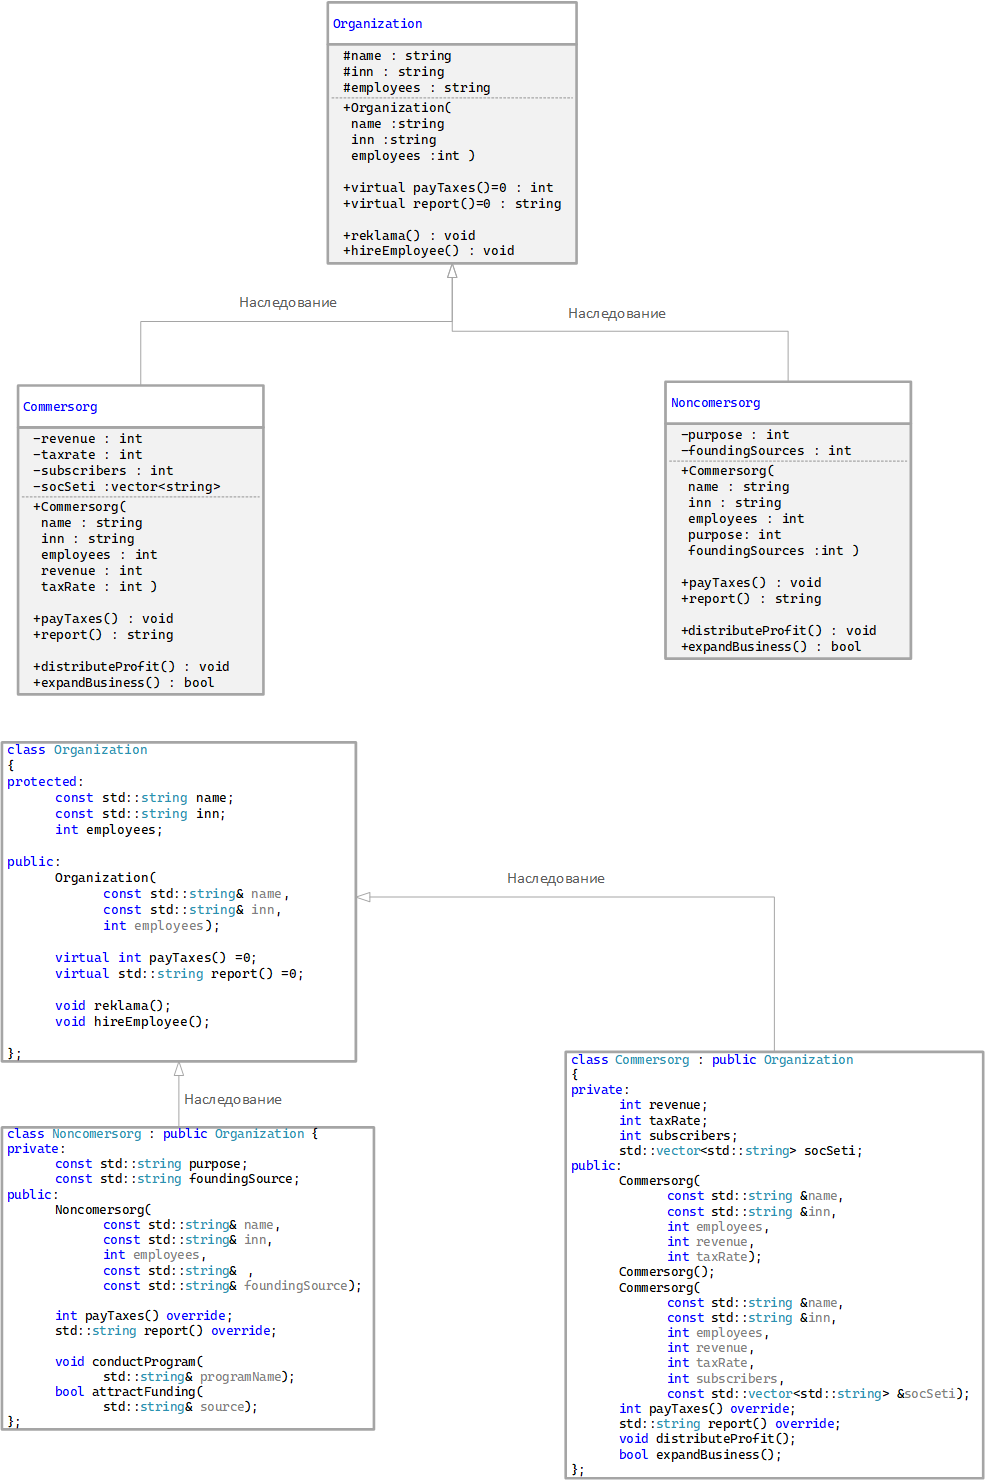
\includegraphics[width=0.8\textwidth]{Диаграмма классов.png}
  \caption{Диаграмма классов}
  \label{fig:landscape}
\end{figure}
% тут картинка интерфейса
\begin{figure}
  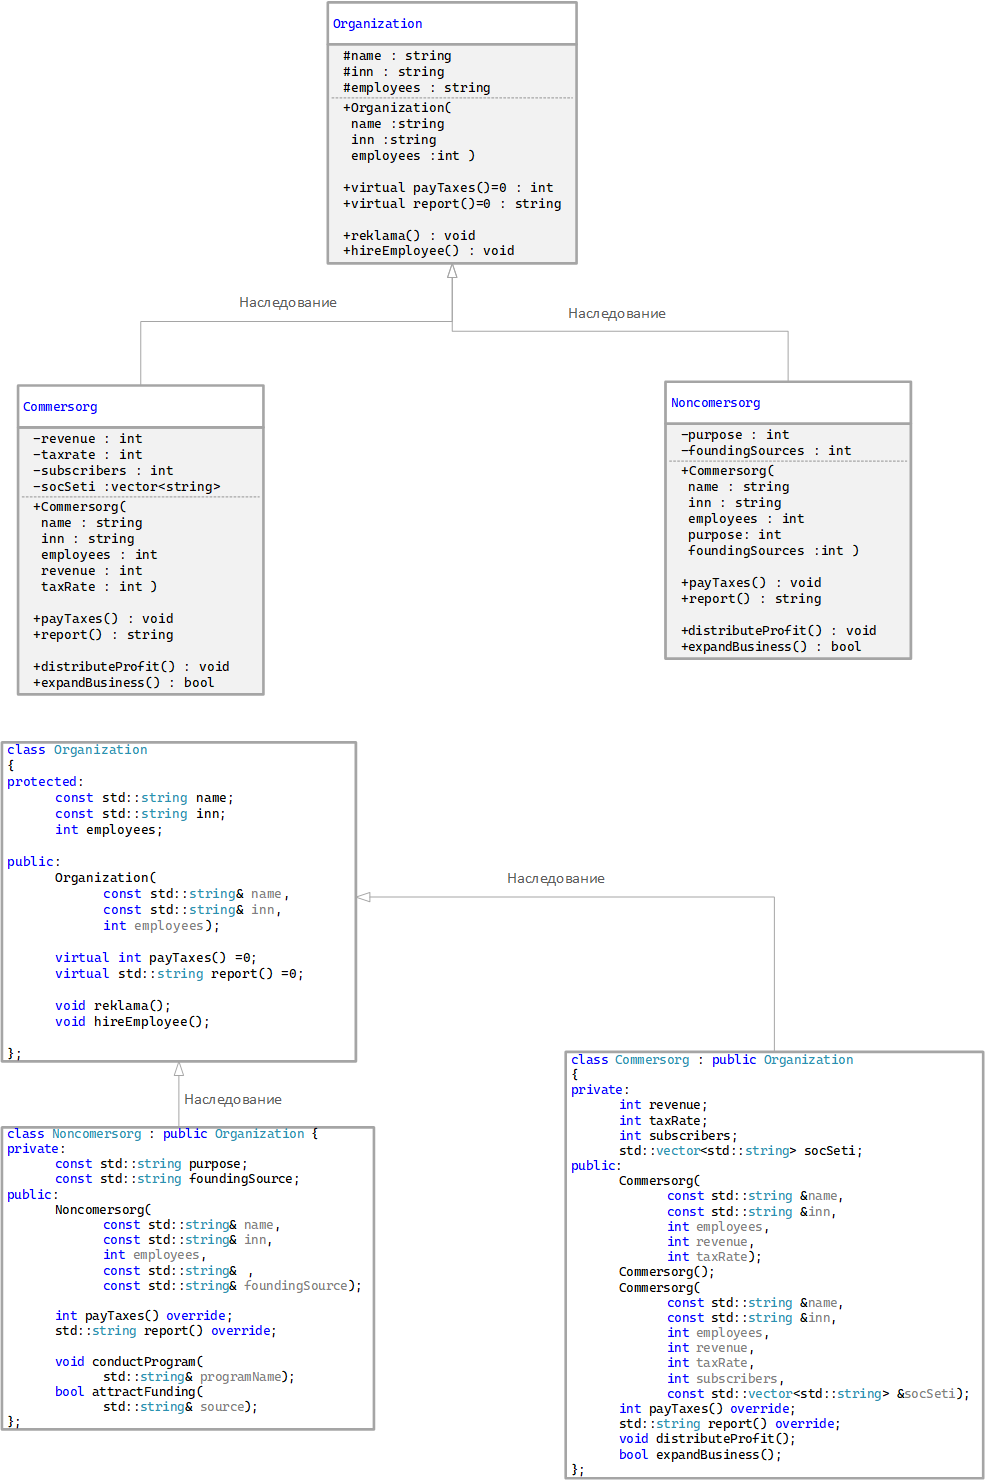
\includegraphics[width=0.8\textwidth]{Диаграмма классов.png}
  \caption{Диаграмма классов}
  \label{fig:landscape}
\end{figure}

\newpage

\subsection*{Особенности подключения и работы с БД PostgreSQL}
\addcontentsline{toc}{subsection}{Особенности подключения и работы с БД PostgreSQL}

Для хранения данных используется СУБД PostgreSQL. Взаимодействие с ней в коде C\# реализовано с помощью библиотеки Npgsql. Согласно требованиям, данные организаций разделены по разным таблицам. Работа с БД имеет следующие особенности:
\begin{itemize}
	\item Разделение таблиц
	 Создана одна главная таблица Organizations для хранения общих полей всех организаций. Для уникальных полей созданы отдельные таблицы ComOrgs и NonComOrgs. Связь между ними настроена через внешний ключ с каскадным удалением, чтобы при удалении из главной таблицы автоматически удалялись связанные данные.
	\item Использование транзакций
	При добавлении или обновлении организации данные нужно записать сразу в две разные таблицы. Чтобы избежать ошибок, когда часть данных сохранилась, а часть нет, эти действия обернуты в транзакции. Если при записи во вторую таблицу произойдет сбой, изменения в первой таблице просто отменятся.
	\item Безопасность запросов
	Чтобы избежать ошибок при вводе данных пользователем, переменные не вставляются в текст SQL-запроса напрямую. Вместо этого используются параметризованные запросы, что гарантирует безопасное сохранение строк.
	\item Чтение данных
	При загрузке списка организаций программа выполняет объединение главной таблицы с дочерними с помощью LEFT JOIN. После получения строки из БД программа проверяет тип организации и на его основе динамически создает нужный объект — коммерческую или некоммерческую организацию.
\end{itemize}

\newpage

\subsection*{Разработка графического интерфейса пользователя}
\addcontentsline{toc}{subsection}{Разработка графического интерфейса}

Приложение разработано с использованием Windows Forms. Главное окно содержит:
\begin{itemize}
    \item Список загруженных организаций.
    \item Блок ввода данных, где расположены текстовые поля. При переключении типа создаваемой организации скрываются ненужные поля и появляются нужные.
    \item Блок операций с БД, содержащий кнопки для добавления, удаления и обновления информации.
    \item Блок методов классов, который позволяет вызывать унаследованные из первой лабораторной работы функции.
\end{itemize}

\section*{Вывод}
\addcontentsline{toc}{section}{Вывод}

В ходе выполнения второй лабораторной работы консольное приложение на C++ было успешно перенесено на язык C\# с созданием графического интерфейса пользователя.

Были выполнены все требования преподавателя:
\begin{enumerate}
    \item Сохранена структура классов из первой лабораторной работы, настроена инкапсуляция через свойства.
    \item Реализован удобный графический интерфейс на Windows Forms, который скрывает ненужные поля и реагирует на выбор пользователя.
    \item Настроено подключение к базе данных PostgreSQL. Проблема наследования в БД решена путем создания нескольких связанных таблиц, а целостность данных обеспечена использованием транзакций и параметризованных запросов.
\end{enumerate}

\end{document}